\documentclass[border=15pt]{standalone}
\usepackage{tikz}
\usetikzlibrary{arrows.meta, calc}
\usepackage[T1]{fontenc}
\usepackage{lmodern}
\usepackage{xcolor}

\definecolor{cBlue}{HTML}{0000CC}
\definecolor{cGreen}{HTML}{008800}
\definecolor{cRed}{HTML}{CC0000}
\definecolor{cGrey}{HTML}{999999}

\begin{document}
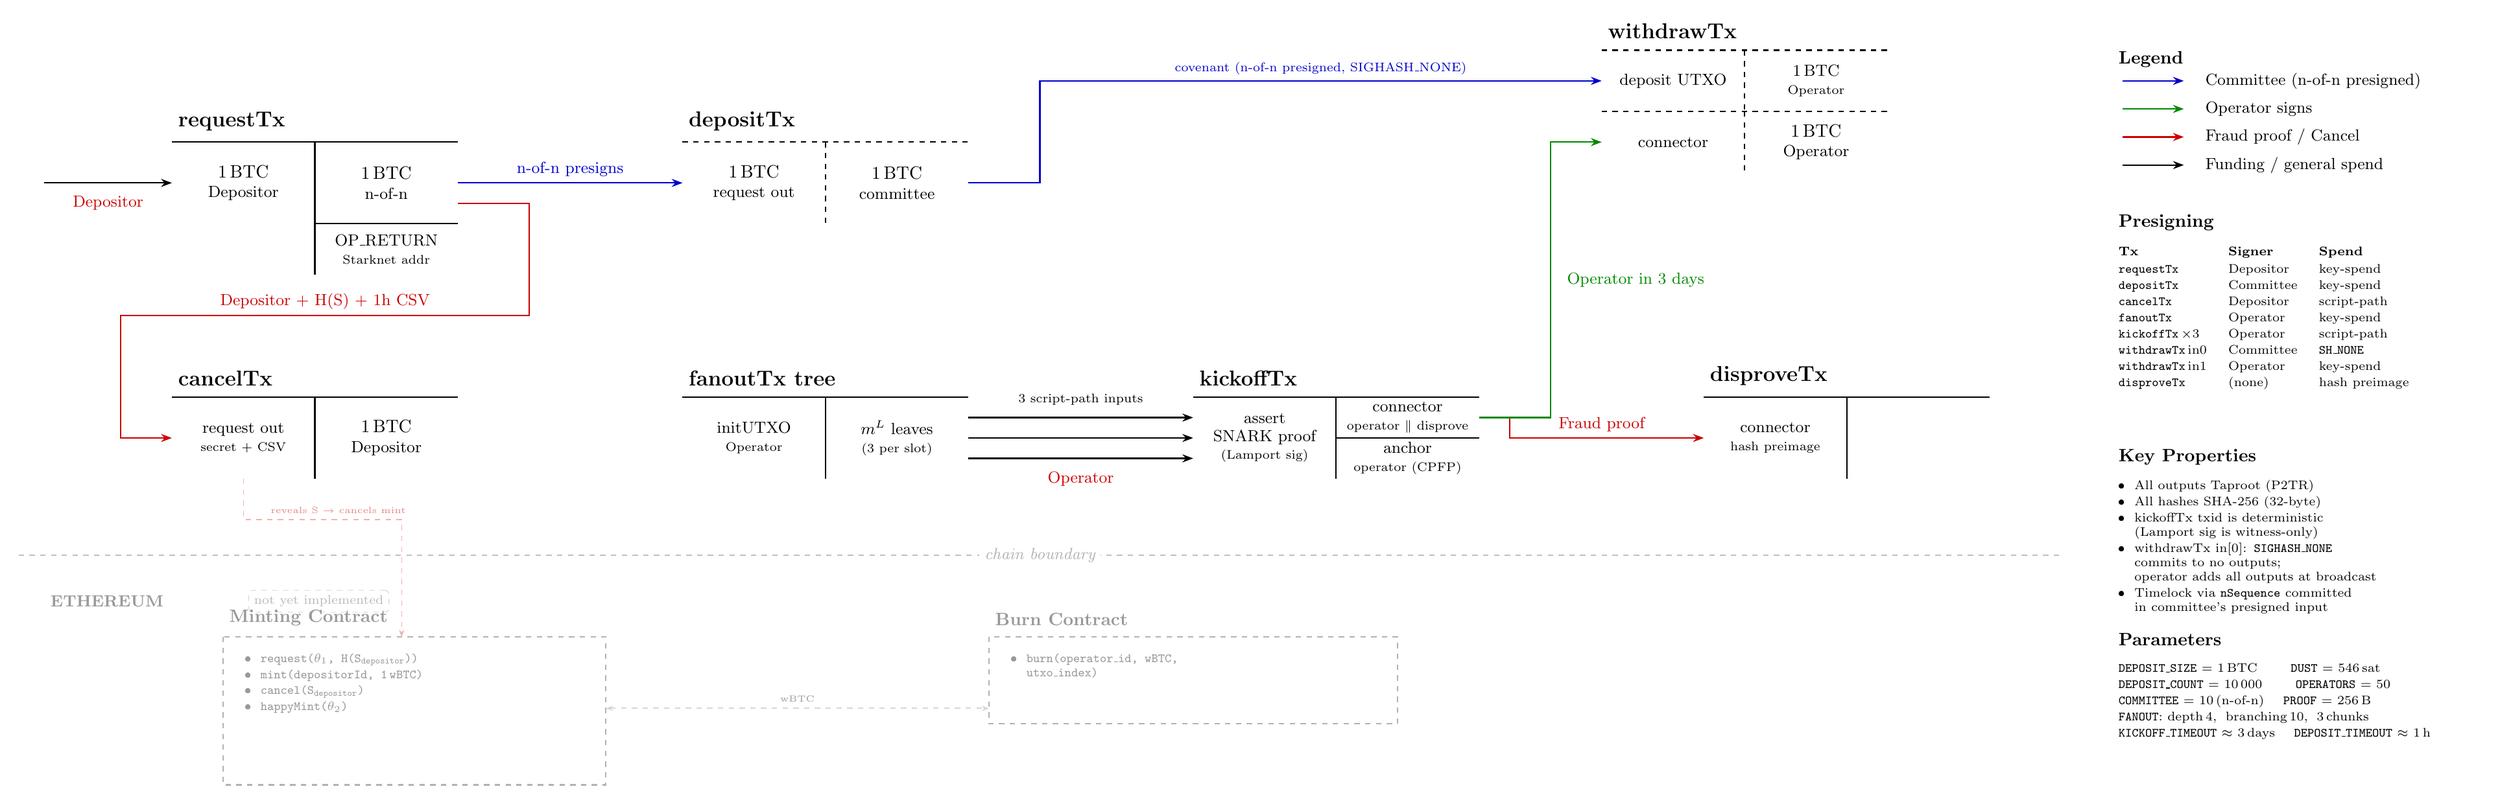
\begin{tikzpicture}[
  txname/.style={font=\bfseries\large, anchor=south west},
  covenant/.style={-{Stealth[length=6pt]}, thick, color=cBlue},
  opspend/.style={-{Stealth[length=6pt]}, thick, color=cGreen},
  fraud/.style={-{Stealth[length=6pt]}, thick, color=cRed},
  plain/.style={-{Stealth[length=6pt]}, thick, color=black},
]

% LAYOUT — two rows of txs, all flowing left→right.
%
% Row 1 (y≈10):  requestTx → depositTx → withdrawTx
% Row 2 (y≈5):   cancelTx ←(from req)   fanoutTx → kickoffTx → disproveTx
%                                          kickoffTx also → withdrawTx (via vertical routing)
%
% STYLE: each tx has ONLY a top-border line and a column-divider line.
%        No left/right/bottom borders.
% ARROWS: enter left col from the left, exit right col to the right.
%         ≥1cm horizontal before any vertical turn.

% Column widths: left col 2.8cm, right col 2.8cm = 5.6cm total per tx
% Row heights: 1.6cm per row


% ══════════════════════════════════════════════════════
%  ROW 1:  requestTx  →  depositTx  →  withdrawTx
%  y: top=10.6, content center=9.8, bottom=9.0
% ══════════════════════════════════════════════════════

% --- requestTx  (x: 0 .. 5.6) ---
\node[txname] at (0, 10.7) {requestTx};
\draw[thick] (0, 10.6) -- (5.6, 10.6);           % top border
\draw[thick] (2.8, 10.6) -- (2.8, 8.0);           % divider (extended for OP_RETURN row)

\node[align=center] at (1.4, 9.8) {1\,BTC\\[-1pt]{\small Depositor}};
\node[align=center] at (4.2, 9.8) {1\,BTC\\[-1pt]{\small n-of-n}};
\draw[thick] (2.8, 9.0) -- (5.6, 9.0);            % right col row divider
\node[align=center, font=\small] at (4.2, 8.5)
  {OP\_RETURN\\[-1pt]{\scriptsize Starknet addr}};

% Depositor funds requestTx (enter left col)
\draw[plain] (-2.5, 9.8) -- (0, 9.8);
\node[font=\small, text=cRed] at (-1.25, 9.4) {Depositor};


% --- depositTx  (x: 10 .. 15.6) ---
\node[txname] at (10, 10.7) {depositTx};
\draw[thick, dashed] (10, 10.6) -- (15.6, 10.6);          % top border
\draw[thick, dashed] (12.8, 10.6) -- (12.8, 9.0);         % divider

\node[align=center] at (11.4, 9.8) {1\,BTC\\[-1pt]{\small request out}};
\node[align=center] at (14.2, 9.8) {1\,BTC\\[-1pt]{\small committee}};

% requestTx → depositTx  (exit right col, enter left col)
\draw[covenant] (5.6, 9.8) -- (10, 9.8);
\node[font=\small, text=cBlue, above] at (7.8, 9.8) {n-of-n presigns};


% --- withdrawTx  (x: 28 .. 33.6) ---
% Two input rows, two output rows
\node[txname] at (28, 12.5) {withdrawTx};

% in[0] row  (y: 12.4 .. 11.2)
\draw[thick, dashed] (28, 12.4) -- (33.6, 12.4);     % top border
\draw[thick, dashed] (30.8, 12.4) -- (30.8, 11.2);   % divider
\node[align=center, font=\small] at (29.4, 11.8)
  {deposit UTXO};
\node[align=center, font=\small] at (32.2, 11.8)
  {1\,BTC\\[-1pt]{\scriptsize Operator}};

% in[1] row  (y: 11.2 .. 10.0)
\draw[thick, dashed] (28, 11.2) -- (33.6, 11.2);     % top border
\draw[thick, dashed] (30.8, 11.2) -- (30.8, 10.0);   % divider
\node[align=center, font=\small] at (29.4, 10.6)
  {connector};
\node[align=center] at (32.2, 10.6) {1\,BTC\\[-1pt]{\small Operator}};

% depositTx → withdrawTx in[0]
% Exit depositTx right col to the right, go ≥1cm, turn up, go right ≥1cm into withdrawTx in[0] left col
\draw[covenant] (15.6, 9.8) -- (17, 9.8) -- (17, 11.8) -- (28, 11.8);
\node[font=\scriptsize, text=cBlue, above, align=center] at (22.5, 11.8)
  {covenant (n-of-n presigned, SIGHASH\_NONE)};


% ══════════════════════════════════════════════════════
%  ROW 2:  cancelTx   fanoutTx → kickoffTx → disproveTx
%  y: top=5.6, content center=4.8, bottom=4.0
% ══════════════════════════════════════════════════════

% --- cancelTx  (x: 0 .. 5.6) ---
\node[txname] at (0, 5.7) {cancelTx};
\draw[thick] (0, 5.6) -- (5.6, 5.6);              % top border
\draw[thick] (2.8, 5.6) -- (2.8, 4.0);            % divider

\node[align=center, font=\small] at (1.4, 4.8)
  {request out\\[-1pt]{\scriptsize secret + CSV}};
\node[align=center] at (4.2, 4.8)
  {1\,BTC\\[-1pt]{\small Depositor}};

% requestTx → cancelTx
% Exit requestTx right col to the right, go 1cm, turn down, go left into cancelTx left col
% requestTx → cancelTx: exit right col → right 1.4cm → down to y=7 → left to x=-1 → down → right into left col
\draw[fraud] (5.6, 9.4) -- (7, 9.4) -- (7, 7.2) -- (-1, 7.2) -- (-1, 4.8) -- (0, 4.8);
\node[font=\small, text=cRed, above] at (3, 7.2)
  {Depositor + H(S) + 1h CSV};


% --- fanoutTx tree  (x: 10 .. 15.6) ---
\node[txname] at (10, 5.7) {fanoutTx tree};
\draw[thick] (10, 5.6) -- (15.6, 5.6);            % top border
\draw[thick] (12.8, 5.6) -- (12.8, 4.0);          % divider

\node[align=center, font=\small] at (11.4, 4.8)
  {initUTXO\\[-1pt]{\scriptsize Operator}};
\node[align=center, font=\small] at (14.2, 4.8)
  {$m^L$ leaves\\[-1pt]{\scriptsize (3 per slot)}};


% --- kickoffTx  (x: 20 .. 25.6) ---
\node[txname] at (20, 5.7) {kickoffTx};
\draw[thick] (20, 5.6) -- (25.6, 5.6);            % top border
\draw[thick] (22.8, 5.6) -- (22.8, 4.0);          % divider
\draw[thick] (22.8, 4.8) -- (25.6, 4.8);          % right col row divider

\node[align=center, font=\small] at (21.4, 4.8)
  {assert\\[-1pt]SNARK proof\\[-1pt]{\scriptsize (Lamport sig)}};
\node[align=center, font=\small] at (24.2, 5.2)
  {connector\\[-1pt]{\scriptsize operator $\|$ disprove}};
\node[align=center, font=\small] at (24.2, 4.4)
  {anchor\\[-1pt]{\scriptsize operator (CPFP)}};

% fanoutTx → kickoffTx  (3 arrows, exit right col, enter left col)
\draw[plain] (15.6, 5.2) -- (20, 5.2);
\draw[plain] (15.6, 4.8) -- (20, 4.8);
\draw[plain] (15.6, 4.4) -- (20, 4.4);
\node[font=\scriptsize] at (17.8, 5.55) {3 script-path inputs};
\node[font=\small, text=cRed] at (17.8, 4.0) {Operator};


% --- disproveTx  (x: 30 .. 35.6) ---
\node[txname] at (30, 5.7) {disproveTx};
\draw[thick] (30, 5.6) -- (35.6, 5.6);            % top border
\draw[thick] (32.8, 5.6) -- (32.8, 4.0);          % divider

\node[align=center, font=\small] at (31.4, 4.8)
  {connector\\[-1pt]{\scriptsize hash preimage}};

% kickoffTx connector → disproveTx  (exit right col connector row, step down to disproveTx)
\draw[fraud] (25.6, 5.2) -- (26.2, 5.2) -- (26.2, 4.8) -- (30, 4.8);
\node[font=\small, text=cRed, above] at (28, 4.8) {Fraud proof};


% ══════════════════════════════════════════════════════
%  kickoffTx connector → withdrawTx in[1]
%  Exit kickoffTx right col → right ≥1cm → up → right ≥1cm → into withdrawTx in[1] left col
% ══════════════════════════════════════════════════════

\draw[opspend] (25.6, 5.2) -- (27, 5.2) -- (27, 10.6) -- (28, 10.6);
\node[font=\small, text=cGreen, anchor=west] at (27.2, 7.9)
  {Operator in 3 days};


% ══════════════════════════════════════════════════════
%  ETHEREUM  (not implemented)
% ══════════════════════════════════════════════════════

\draw[thick, dashed, black!25] (-3, 2.5) -- (37, 2.5);
\node[font=\itshape\small, text=black!30, fill=white, inner sep=3pt]
  at (17, 2.5) {chain boundary};

\node[font=\bfseries\small, text=cGrey, anchor=west]
  at (-2.5, 1.6) {ETHEREUM};
\node[font=\scriptsize, text=cGrey!70,
  draw=cGrey!40, dashed, rounded corners=2pt,
  inner sep=3pt, anchor=west] at (1.5, 1.6)
  {not yet implemented};

% Minting Contract
\node[font=\bfseries\normalsize, text=cGrey, anchor=south west]
  at (1, 1.0) {Minting Contract};
\draw[thick, dashed, black!30] (1, 0.9) rectangle (8.5, -2.0);
\node[font=\scriptsize, text=cGrey, anchor=north west, align=left]
  at (1.3, 0.7) {%
  \textbullet\; \texttt{request($\theta_1$, H(S\textsubscript{depositor}))}\\[1pt]
  \textbullet\; \texttt{mint(depositorId, 1\,wBTC)}\\[1pt]
  \textbullet\; \texttt{cancel(S\textsubscript{depositor})}\\[1pt]
  \textbullet\; \texttt{happyMint($\theta_2$)}};

% Burn Contract
\node[font=\bfseries\normalsize, text=cGrey, anchor=south west]
  at (16, 1.0) {Burn Contract};
\draw[thick, dashed, black!30] (16, 0.9) rectangle (24, -0.8);
\node[font=\scriptsize, text=cGrey, anchor=north west, align=left]
  at (16.3, 0.7) {%
  \textbullet\; \texttt{burn(operator\_id, wBTC,}\\
  \phantom{\textbullet\;} \texttt{utxo\_index)}};

% wBTC arrow
\draw[thick, dashed, cGrey!40,
  {Stealth[length=4pt]}-{Stealth[length=4pt]}]
  (8.5, -0.5) --
  node[font=\tiny, text=cGrey, above]{wBTC}
  (16, -0.5);

% Cross-chain: cancel → cancels mint
\draw[dashed, cRed!30, -{Stealth[length=4pt]}]
  (1.4, 4.0) -- (1.4, 3.2)
  -- node[font=\tiny, text=cRed!50, above, pos=0.6]
    {reveals S $\rightarrow$ cancels mint}
  (4.5, 3.2) -- (4.5, 0.9);



% ══════════════════════════════════════════════════════
%  RIGHT PANEL — Legend, Presigning, Key Properties, Parameters
% ══════════════════════════════════════════════════════

\begin{scope}[shift={(38, 12.5)}]

  \node[font=\bfseries\normalsize, anchor=north west] at (0, 0) {Legend};

  \draw[covenant] (0.2, -0.7) -- (1.4, -0.7);
  \node[font=\small, anchor=west] at (1.7, -0.7)
    {Committee (n-of-n presigned)};

  \draw[opspend] (0.2, -1.25) -- (1.4, -1.25);
  \node[font=\small, anchor=west] at (1.7, -1.25)
    {Operator signs};

  \draw[fraud] (0.2, -1.8) -- (1.4, -1.8);
  \node[font=\small, anchor=west] at (1.7, -1.8)
    {Fraud proof / Cancel};

  \draw[plain] (0.2, -2.35) -- (1.4, -2.35);
  \node[font=\small, anchor=west] at (1.7, -2.35)
    {Funding / general spend};

  \node[font=\bfseries\normalsize, anchor=north west] at (0, -3.2) {Presigning};
  \node[font=\scriptsize, anchor=north west] at (0, -3.8) {%
    \begin{tabular}{@{}lll@{}}
    \textbf{Tx} & \textbf{Signer} & \textbf{Spend} \\[2pt]
    \texttt{requestTx}            & Depositor & key-spend \\[1pt]
    \texttt{depositTx}            & Committee & key-spend \\[1pt]
    \texttt{cancelTx}             & Depositor & script-path \\[1pt]
    \texttt{fanoutTx}             & Operator  & key-spend \\[1pt]
    \texttt{kickoffTx}\,$\times$3 & Operator  & script-path \\[1pt]
    \texttt{withdrawTx}\,in0      & Committee & \texttt{SH\_NONE} \\[1pt]
    \texttt{withdrawTx}\,in1      & Operator  & key-spend \\[1pt]
    \texttt{disproveTx}           & (none)    & hash preimage \\
    \end{tabular}};

  \node[font=\bfseries\normalsize, anchor=north west] at (0, -7.8) {Key Properties};
  \node[font=\scriptsize, anchor=north west, text width=7cm] at (0, -8.4) {%
    \textbullet\; All outputs Taproot (P2TR)\\[1pt]
    \textbullet\; All hashes SHA-256 (32-byte)\\[1pt]
    \textbullet\; kickoffTx txid is deterministic\\
    \phantom{\textbullet}\; (Lamport sig is witness-only)\\[1pt]
    \textbullet\; withdrawTx in[0]: \texttt{SIGHASH\_NONE}\\
    \phantom{\textbullet}\; commits to no outputs;\\
    \phantom{\textbullet}\; operator adds all outputs at broadcast\\[1pt]
    \textbullet\; Timelock via \texttt{nSequence} committed\\
    \phantom{\textbullet}\; in committee's presigned input};

  \node[font=\bfseries\normalsize, anchor=north west] at (0, -11.4) {Parameters};
  \node[font=\scriptsize, anchor=north west, text width=7cm] at (0, -12.0) {%
    \texttt{DEPOSIT\_SIZE} = 1\,BTC \qquad
    \texttt{DUST} = 546\,sat\\[1pt]
    \texttt{DEPOSIT\_COUNT} = 10\,000 \qquad
    \texttt{OPERATORS} = 50\\[1pt]
    \texttt{COMMITTEE} = 10\,(n-of-n) \quad
    \texttt{PROOF} = 256\,B\\[1pt]
    \texttt{FANOUT}: depth\,4,\; branching\,10,\; 3\,chunks\\[1pt]
    \texttt{KICKOFF\_TIMEOUT} $\approx$ 3\,days \quad
    \texttt{DEPOSIT\_TIMEOUT} $\approx$ 1\,h};

\end{scope}

\end{tikzpicture}
\end{document}
